\section{Introduction}
\label{sec:intro}

\begin{figure}[t]
\centering
  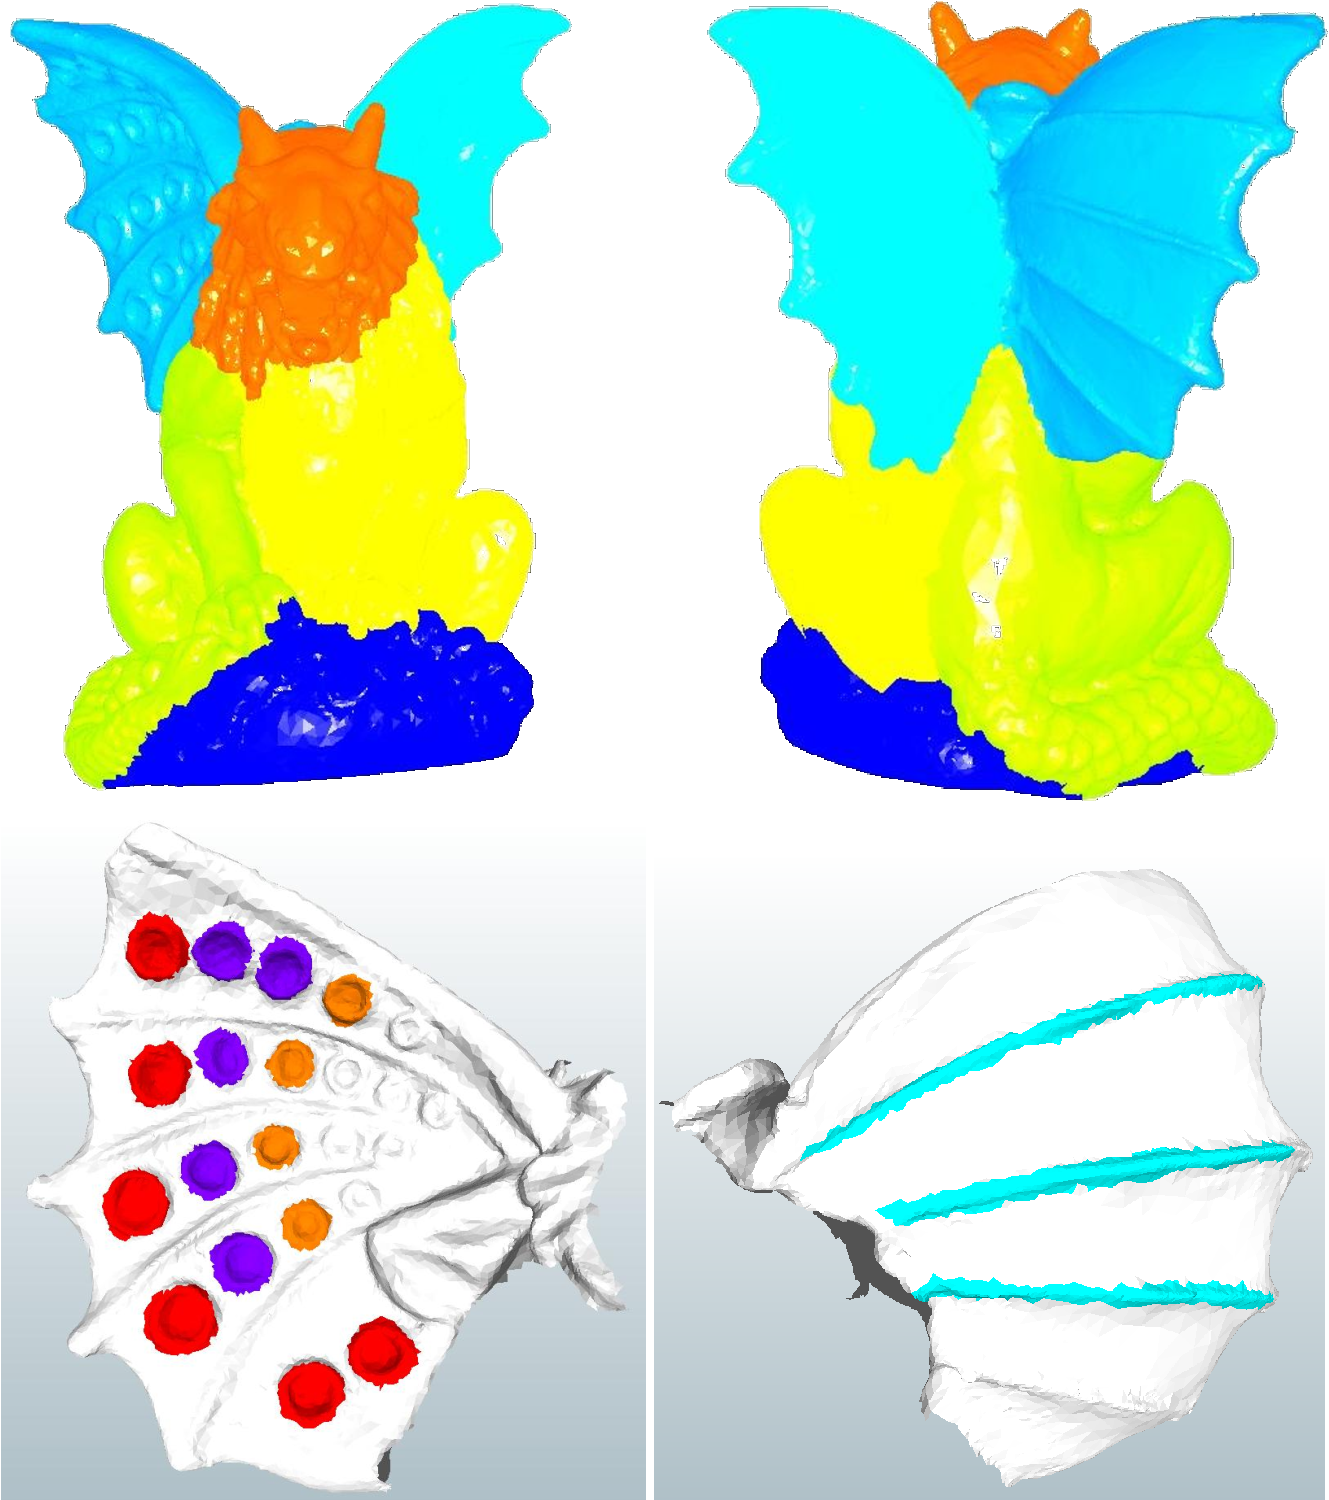
\includegraphics[width=0.99\linewidth]{figures/Gargoyl.pdf}
  \caption{Two-scale symmetries of Gargoyl status from two viewpoints.
  Top: coarse-scale two pairs of mirroring symmetry from six segmented parts are represented, each pair is rendered by similar color.
  Below: fine-scale translation and rotation symmetry detections for the detailed rings.}
\label{fig:Gargoyl}
\end{figure}

Many objects, both man-made and natural, have some symmetries or self-similarities in them.
Finding the symmetry from triangle meshes is a way to augment meshes with some structures thus helps various applications such as remeshing~\cite{podolak2006}, mesh simplification~\cite{pauly2008}, segmentation~\cite{mitra2006,xu2009}, repairing~\cite{bokeloh2009,berner2011}, and reconstruction~\cite{zabrodsky1997}.
Symmetry detection and analysis is a fundamental technique in the computer graphics, computer vision and geometry processing.
Whilst a lot of attention has been received in recent years, it is still challenging to robustly identify symmetries in general input meshes without resorting to user assistance.

Symmetries may have different definitions. In this work, we focus on generalized partial symmetry~\cite{mitra2006,berner2011} where some subset of a shape that reoccurs multiple times within the model differing by combination of translation, rotation or mirroring. Intrinsic symmetries are also considered in which case further isometric deformation is allowed between copies. This flexible definition allows symmetry detection to be more useful.

In this paper, we propose an effective method for generalized partial symmetry detection.
The input mesh is first segmented into multiple meaningful pieces. The correspondence between every pair of pieces
is established using a matching and any pair with significantly high number of correspondences is recognized as a symmetric pair.

Compared to the recent graph matching algorithms~\cite{bokeloh2009,berner2011} based on the salient lines, our algorithm could produce more robust partial symmetry detection results.
As shown by Figure~\ref{fig:Gargoyl}, the two-scale symmetries of the Gargoyl status are correctly detected, which is the failure case of~\cite{berner2011}.
The top is the coarse-scale mirroring symmetry detection from six meaningful segmented parts, two pairs mirroring symmetries (represented by similar colors) have been found.
The below is the fine-scale symmetry detection on the left wing, both the translational and rotational symmetries have been found for the detailed rings.    

The rest of the paper is structured as follows. After the related algorithms are surveyed in Section 2, Section 3 describes our symmetry detection algorithm. 
Section 4 demonstrates some results and compares them with related works. Finally, section 5 makes conclusions and gives some discussions and future directions. 